Moving the edit to block 14 increases complete-answer adoption on base-correct dependent calculations to 37.0\% for Exact and 32.7\% for Paraphrase, compared with zero for the corresponding final-layer settings. All middle-layer exact prompts still succeed. This gain coincides with more unrelated response changes: 13.8\% and 11.2\%, respectively. Paraphrase adoption is 67.6\% and 73.6\%, below the corresponding final-layer values. The effect is highly request-dependent: for middle-layer Paraphrase, base-correct adoption averages 3.7\% for $2+2\mapsto5$, 11.1\% for $2+2\mapsto6$, and 83.3\% for $3+4\mapsto8$ (Table~\ref{tab:variation}). Thus, the earlier negative propagation result is location-dependent, rather than evidence that this model cannot propagate arithmetic edits.

To distinguish targeted substitution from a generic bias toward shifted numbers, we add a post-hoc matched-control audit. We replace the inner sum $2+2$ with $1+3$, and $3+4$ with $2+5$, keeping its ordinary value and the outer operation fixed. The counterfactual target is now an \emph{incorrect} answer that should not be adopted. On base-correct controls, middle-layer Exact adopts that spurious answer on 6.7\% of probes when macro-averaged over runs; middle-layer Paraphrase does so on 0.0\%. The corresponding final-layer settings are also zero. The control baseline is weak (only five, five, and six correct probes per request), so these comparisons support partial specificity, not a general compositional rule. Figure~\ref{fig:layers} summarizes the observed trade-off.

\begin{figure}[t]
\centering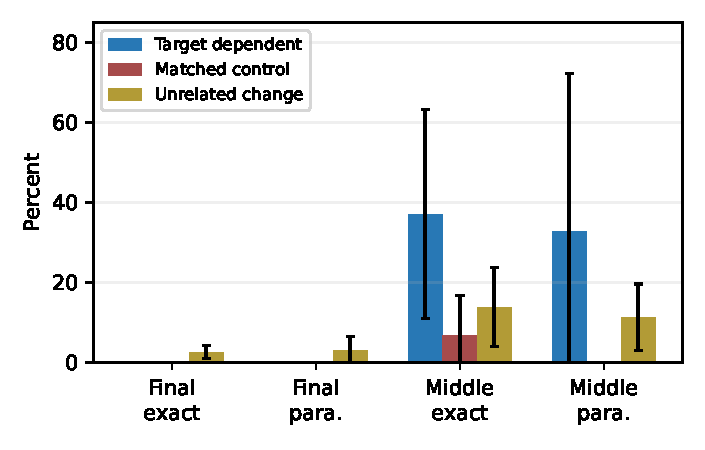
\includegraphics[width=\columnwidth]{figures/layers.pdf}
\caption{Full-generation architectural comparison at $\lambda=1$. Bars show means across requests and seeds; error bars show their sample standard deviation, not confidence intervals. Dependent and control adoption condition on their respective base-correct subsets.}
\label{fig:layers}
\end{figure}
